\section{Early phase \texorpdfstring{\yp{}}{Y. pestis} infection}

\yp{} differs from its evolutionary antecedent, \textit{Y.~pseudotuberculosis},
in a few ways, but one stands out. \yp{} exhibits two phases in its
pathogenesis of mammalian hosts. In the first, the bacteria are readily
absorbed by host leucocytes via phagocytosis --- white blood cells, mainly
macrophages and neutrophils --- and within macrophages especially they
replicate in relative shelter and secrecy from patrolling immune agents. In the
second, after a switching period, they prevent this absorption by a combination
of shielding and active interference. This work explores the mathematical
implications of the switching in an attempt to quantify the significance of the
strategy's evolutionary advantage.

\begin{figure}[h!]
\centering
\begin{subfigure}[b]{0.30\textwidth}
\centering
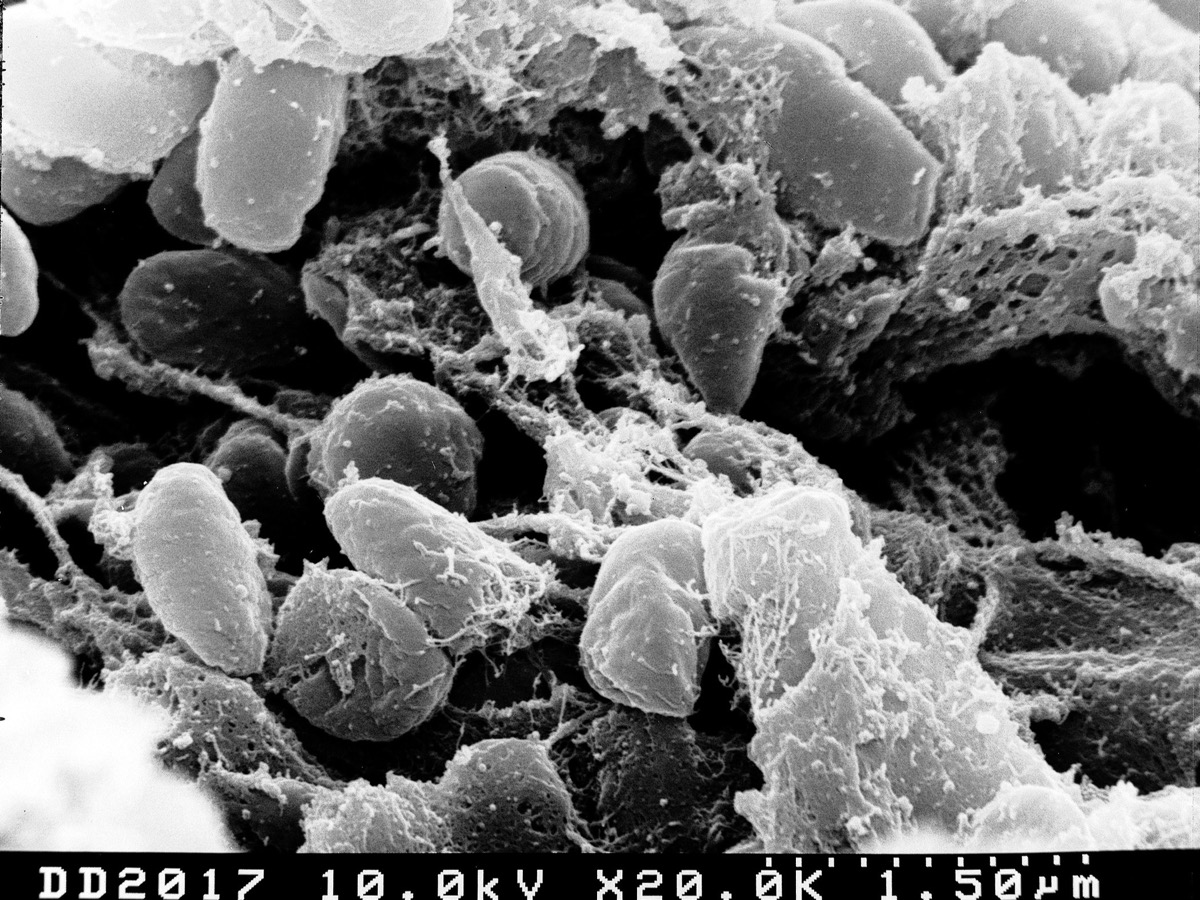
\includegraphics[height=3.35cm]{figures/fig_yp_micrographs/yp_sem_flea}
\caption*{(a) In the flea foregut.}
\end{subfigure}
\hfill
\begin{subfigure}[b]{0.36\textwidth}
\centering
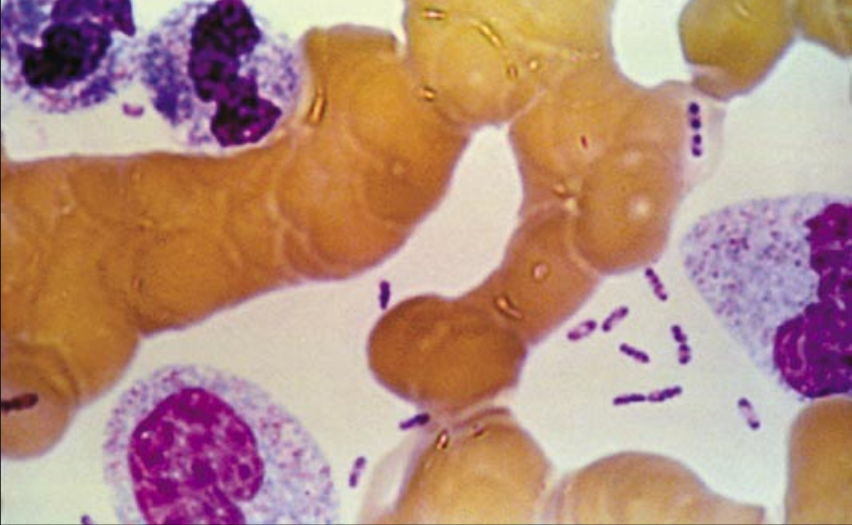
\includegraphics[height=3.35cm]{figures/fig_yp_micrographs/yp_wayson_hi}
\caption*{(b) Wayson stain.}
\end{subfigure}
\hfill
\begin{subfigure}[b]{0.26\textwidth}
\centering
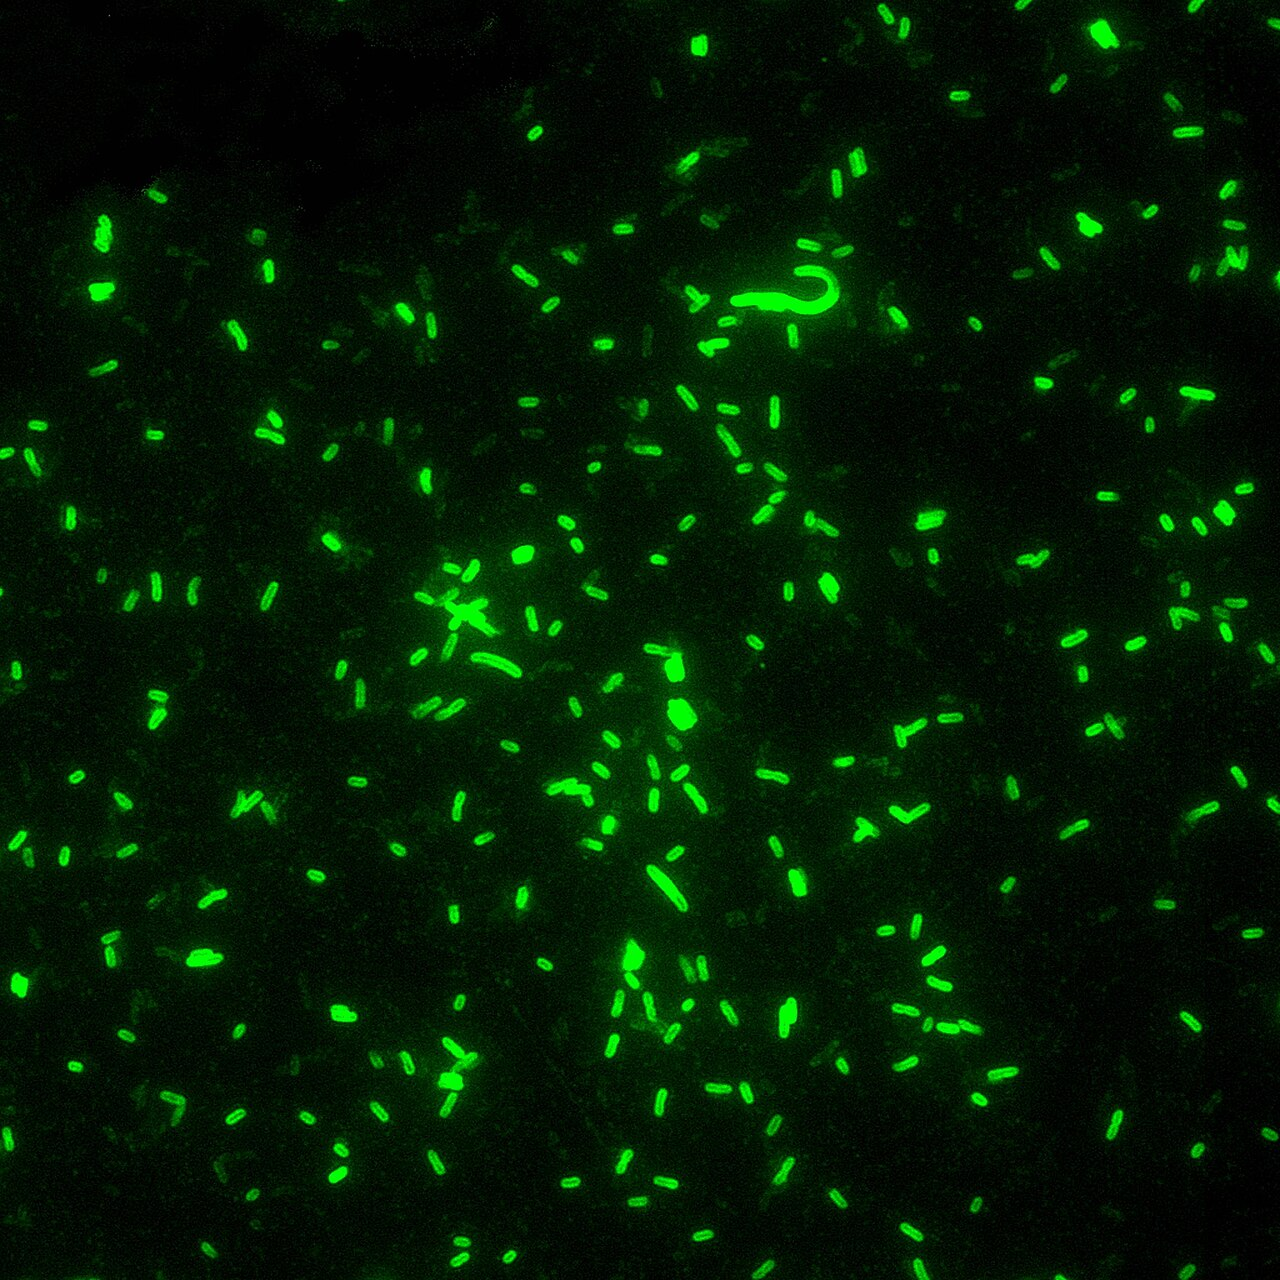
\includegraphics[height=3.35cm]{figures/fig_yp_micrographs/yp_dfa_field}
\caption*{(c) Antibody stain.}
\end{subfigure}
\caption{The organism. (a) Scanning electron micrograph of \yp{} massed in the
foregut of a flea, where the bacteria form the biofilm blockage that makes the
vector infectious; the scale bar in the original reads $1.5\,\mu$m. (b) Wayson
stain, showing the bipolar ``safety pin'' appearance by which the bacillus is
recognised, scattered among host leucocytes. (c) Direct fluorescent antibody
stain, in which the antibody binds the F1 capsular antigen --- one of the
phase-two factors described below, and absent at flea temperature; the field
gives a fair impression of the numbers involved. Sources: (a)~NIAID;
(b)~and~(c) CDC Public Health Image Library. All three are in the public
domain.}
\label{fig:yp_micrographs}
\end{figure}

\subsubsection*{Phase one: an unarmed inoculum, and a permissive compartment}

The bacterium that arrives in a mammalian host is not the bacterium that later
dominates it. In the classical bubonic cycle \yp{} multiplies in the flea
midgut at roughly ambient temperature, and at that temperature it produces
little or none of the F1 capsule, while much of the temperature-induced
mammalian virulence package is not fully on \cite{KeEtAl2013}. What a flea bite
delivers into the dermis is therefore a vector-adapted population, unarmed for
the host it has just entered. Most bacilli that encounter neutrophils at the
bite site are killed; a minority are phagocytosed by tissue macrophages, which
fail to sterilise the infection and instead supply a protected niche.

Inside the macrophage the bacteria occupy a specialised compartment, the
\textit{Yersinia}-containing vacuole. Rather than being delivered efficiently
to a fully bactericidal phagolysosome, this vacuole remains spacious and
relatively permissive, with acidification and autophagic killing both limited
\cite{PujolBliska2005,ConnorEtAl2018}. Within it the organism multiplies and
experiences a suite of host-associated stresses --- body temperature, reduced
pH, oxidative pressure, restricted metal availability. These do more than
select for hardy cells; they act as signals which rewire gene expression, and
the intracellular interval buys the time needed to synthesise the machinery
that will define the second phase. The macrophage is as much a developmental
window as a refuge.

\subsubsection*{Phase two: a surface that refuses re-entry}

Temperature is the master cue. A shift from about $26\text{--}28^\circ$C to
$37^\circ$C induces the F1 capsule, components of the type III secretion
system, and many other virulence loci besides; the mildly acidic pH encountered
in the vacuole specifically favours the pH~6 antigen \cite{KeEtAl2013}. Three
classes of factor matter most. The F1 capsule, assembled as linear fibres over
the cell surface, interferes with uptake and sterically masks the shorter
adhesins that promoted entry in the first place. The pH~6 antigen promotes
attachment in a way that does not efficiently trigger internalisation. And the
Ysc--Yop type III secretion system, on contact with a host cell, injects
effector proteins directly into the eukaryotic cytosol: YopH disrupts the
focal-adhesion signalling required for phagocytic uptake, while YopE, YopT and
YpkA between them disable the Rho-family signalling that organises the actin
cytoskeleton. Together these paralyse phagocytosis. The same cell that earlier
needed invasive factors to enter a macrophage now presents a surface optimised
to refuse re-entry.

\subsubsection*{Why not begin in phase two?}

If the anti-phagocytic state is what enables explosive extracellular growth,
why does the organism not arrive already in it? The literature gives several
reasons, and they are not exclusive \cite{KeEtAl2013,PujolBliska2005}. Under
natural transmission phase two is simply unavailable at the moment of
inoculation, because the flea is cool and the programme is temperature-cued.
Even once the cue is received, reprogramming is not instantaneous --- capsule
assembly and build-up of the secretion apparatus take hours --- and neutrophils
do not wait. The two surfaces are partly antagonistic, so a bacterium
presenting a full phase-two coat would impair the very macrophage entry which,
under natural transmission, supplies the window in which to adapt. And a
permanently assembled secretion system is metabolically expensive, and of no
use at all in the flea.

Those are reasons why the sequence is \emph{forced}. They leave open the
separate question this thesis is about: granted that the sequence is forced, is
it also worth something? Does passing through a protected compartment and
arriving outside in numbers improve the odds of establishment by enough to
matter, and if so, by how much?

\subsubsection*{The sequence in outline}

At the outset of invasion, colony forming units are phagocytosed by host
macrophages, and with evolved resistance to their toxins the bacteria use this
intracellular refuge as a temporary home in which to replicate and bolster
numbers against challenges to come. The first mounted attack of the innate immune system is
neutrophils. Summoned by various cytokines, they arrive on the scene in
numbers, passing through the walls of blood vessels into the extracellular
matrix in which the infection is beginning to take hold. After some time an
infected macrophage will rupture and its resident bacterial population will
disperse. Those \yp{} bacteria which have undergone the transition to the
second phase are characterised by being resistant to further phagocytosis.
Figure~\ref{fig:two_columns_six_image} illustrates the dynamics.

\begin{figure}[h!]
\centering
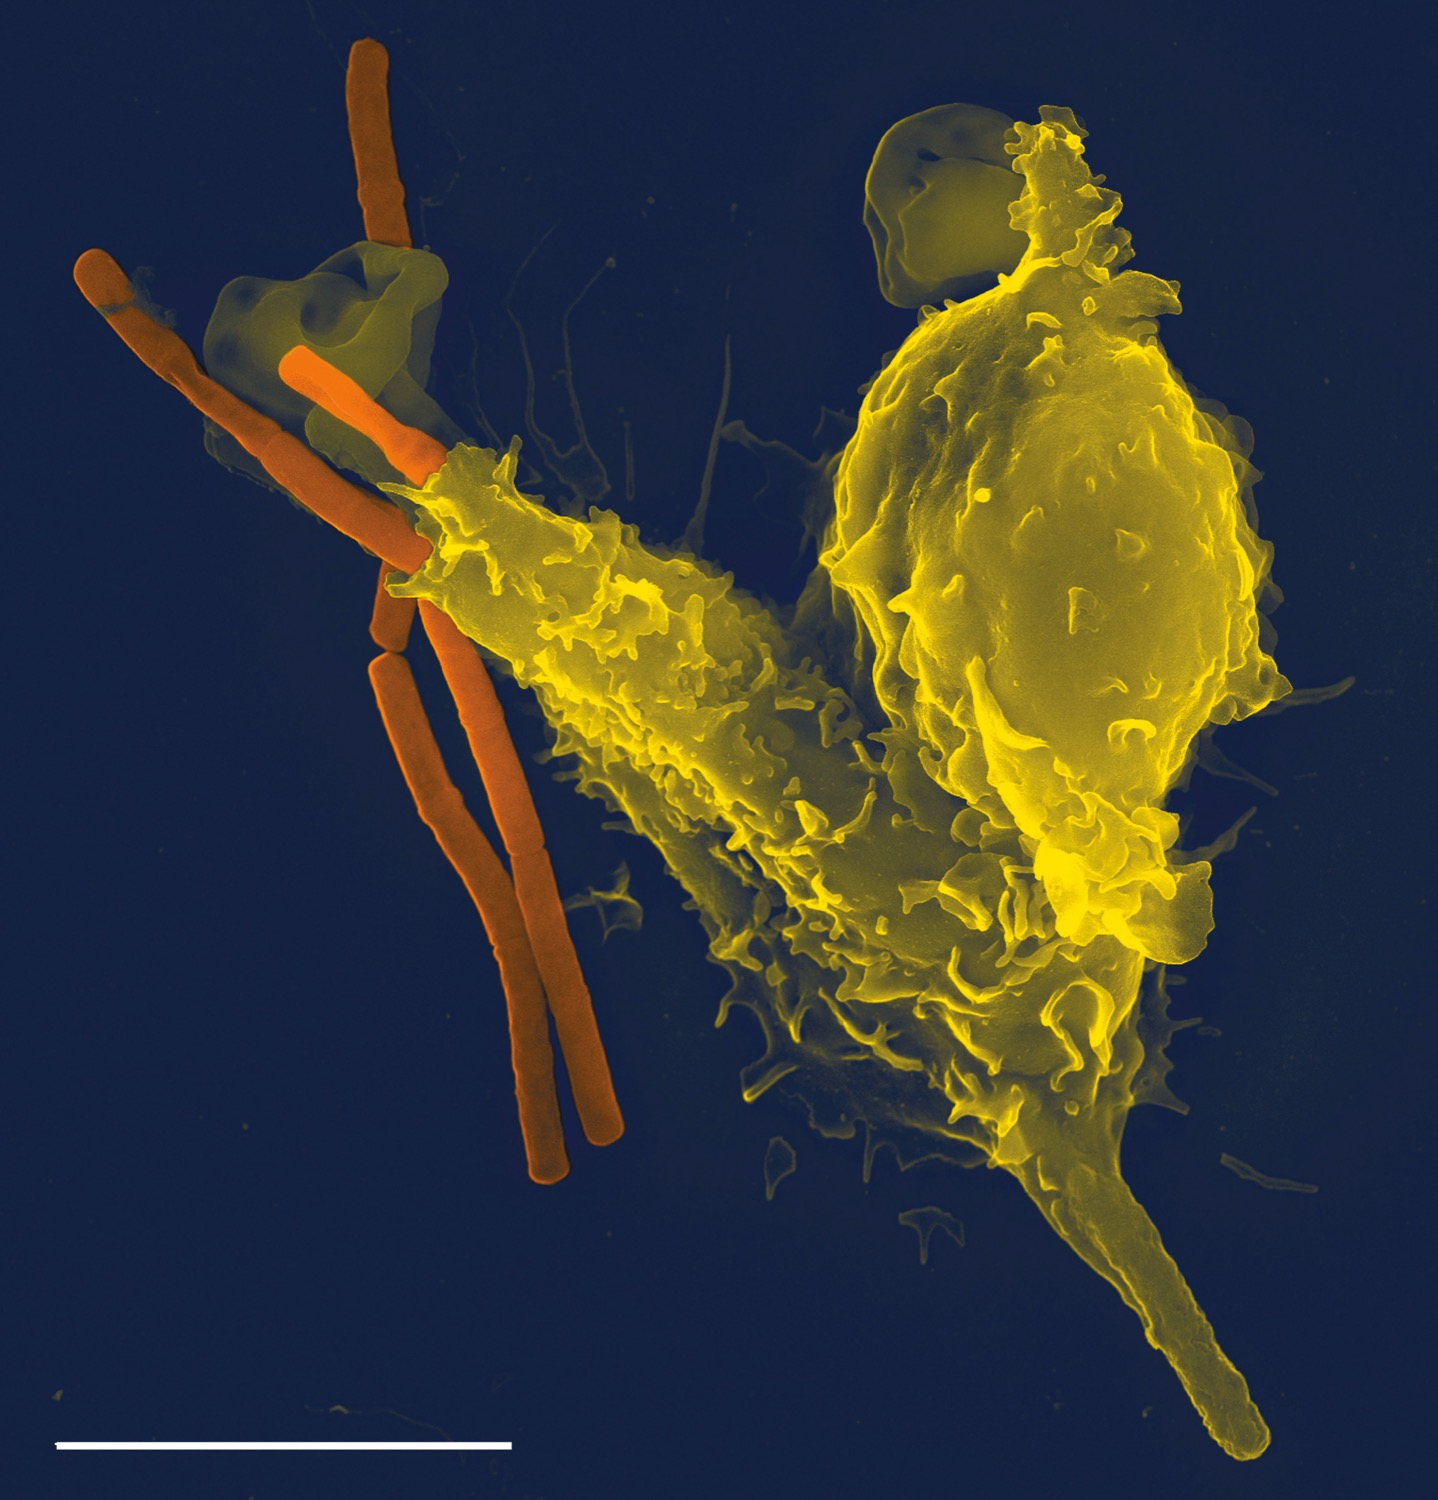
\includegraphics[width=0.52\textwidth]{figures/fig_phagocytosis/neutrophil_anthrax}
\caption{Phagocytosis, the act on which the whole strategy turns. A neutrophil
(yellow) engulfing bacilli (orange); the scale bar is $5\,\mu$m. This is what
\yp{} permits in its first phase and refuses in its second, and it is what the
injected effectors YopH, YopE, YopT and YpkA exist to prevent. The bacteria
shown are \textit{Bacillus anthracis} rather than \yp{}. Image by Volker
Brinkmann, cover of \textit{PLoS Pathogens} 1(3), 2005, reproduced under
CC~BY~2.5.}
\label{fig:phagocytosis}
\end{figure}


\begin{figure}[h!]
    \centering
    % First row of two images
    \begin{subfigure}{0.48\textwidth}
        \centering
        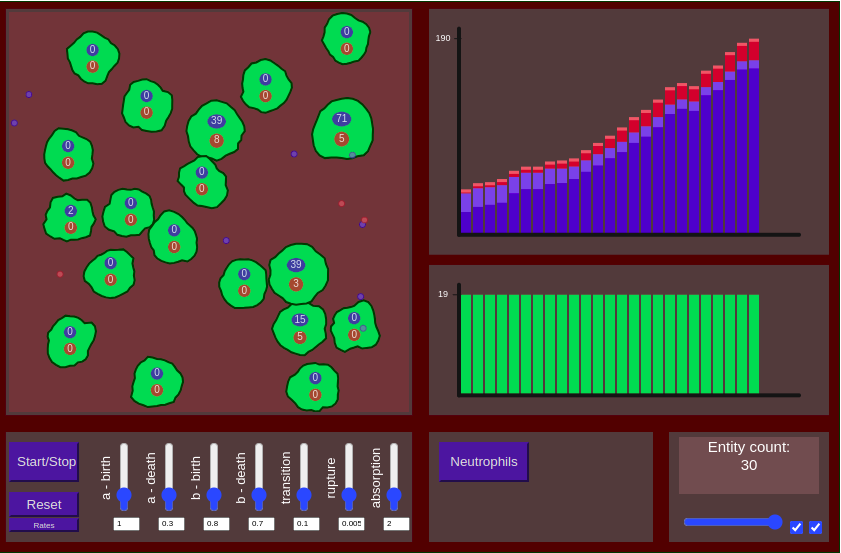
\includegraphics[width=\textwidth]{figures/fig_yp_schematic/web1}
    \end{subfigure}
    \hspace{\fill}
    \begin{subfigure}{0.48\textwidth}
        \centering
        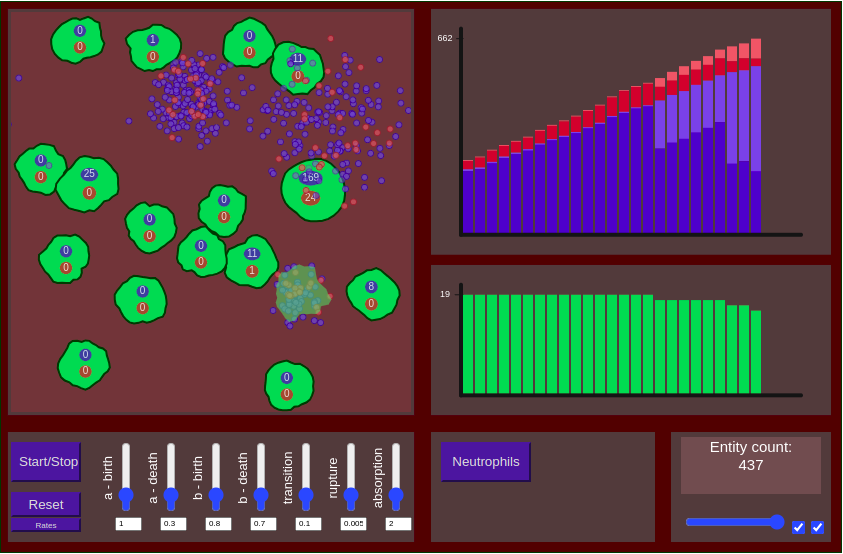
\includegraphics[width=\textwidth]{figures/fig_yp_schematic/web2}
    \end{subfigure}

\caption*{Bacterial replication takes place within the macrophage. Some phase transitions occur.}
    \vspace{0.5em} % Small vertical space between rows

    % Second row of two images
    \begin{subfigure}{0.48\textwidth}
        \centering
        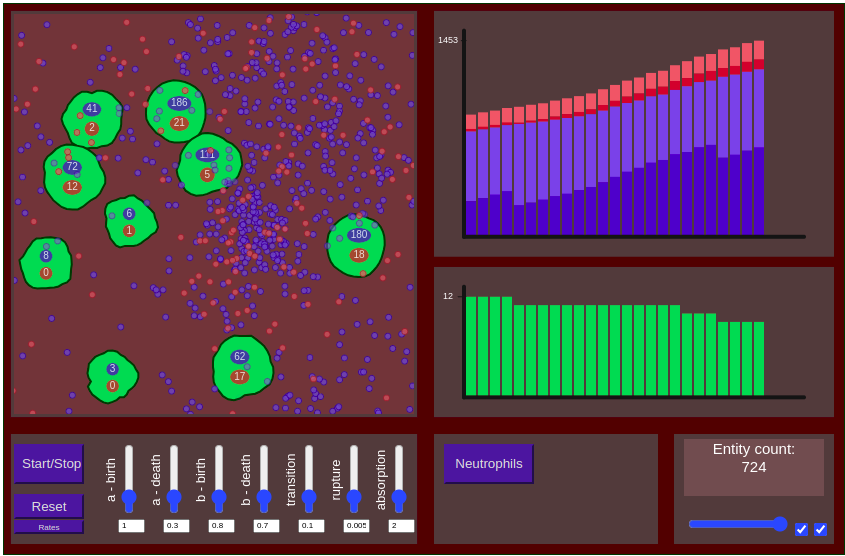
\includegraphics[width=\textwidth]{figures/fig_yp_schematic/web3}
    \end{subfigure}
    \hspace{\fill}
    \begin{subfigure}{0.48\textwidth}
        \centering
        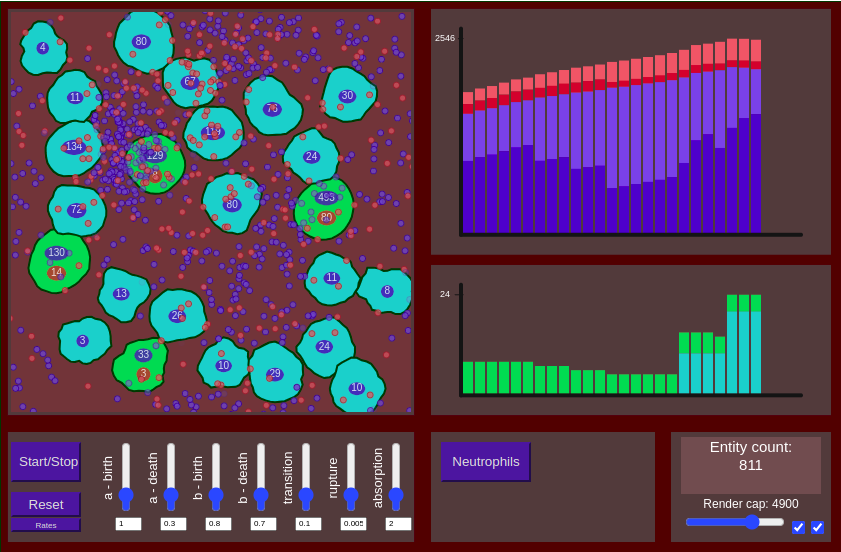
\includegraphics[width=\textwidth]{figures/fig_yp_schematic/web4}
    \end{subfigure}

\caption*{The macrophage bursts; more transitions to the second phase (red particles). Neutrophils arrive.}
    \vspace{0.5em} % Small vertical space between rows

    % Third row of two images
    \begin{subfigure}{0.48\textwidth}
        \centering
        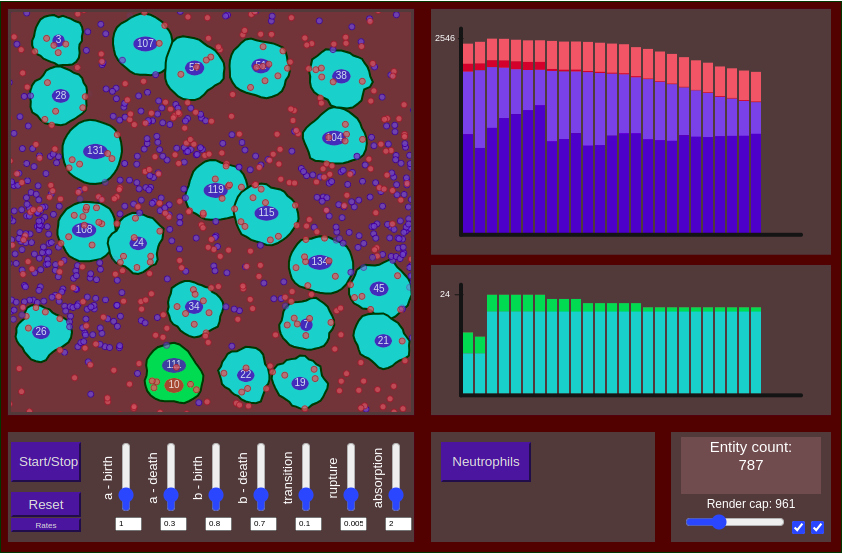
\includegraphics[width=\textwidth]{figures/fig_yp_schematic/web5}
    \end{subfigure}
    \hspace{\fill}
    \begin{subfigure}{0.48\textwidth}
        \centering
        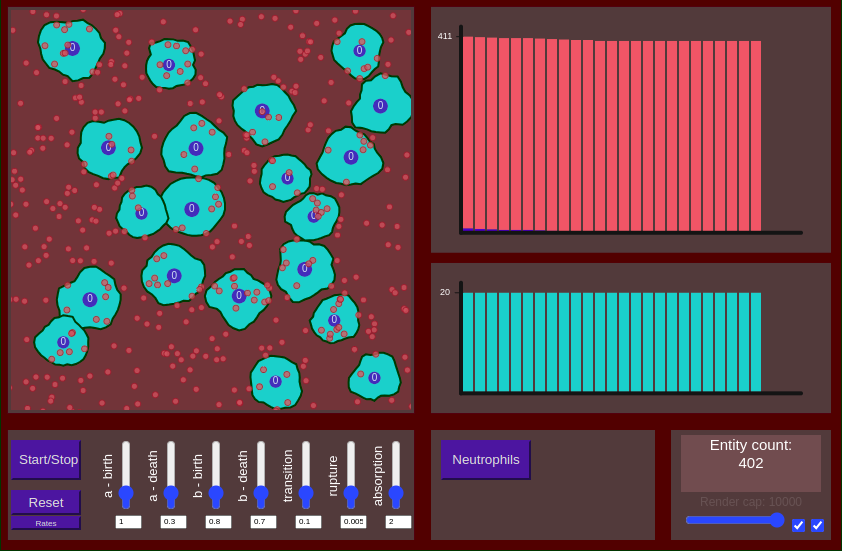
\includegraphics[width=\textwidth]{figures/fig_yp_schematic/web6}
    \end{subfigure}

    % Single caption for all images
\caption*{Neutrophils phagocytose and eliminate the remaining phase one bacteria, leaving \yp{} as a primarily extracellular infection.}
    \caption{A schematic representation.}
    \label{fig:two_columns_six_image}
\end{figure}

\subsubsection*{The exit, which is not settled}

Teaching summaries put the last step of that sequence bluntly: the bacteria
replicate inside macrophages, the macrophages burst, and free bacilli spread.
The primary literature is more careful. Phase-two machinery certainly can kill
macrophages --- YopJ-dependent apoptosis is well supported
\cite{MonackEtAl1997}, in activated macrophages the infection can be redirected
towards caspase-1-dependent pyroptosis, and necroptosis of infiltrated
macrophages has been proposed to promote dissemination in lymph nodes
\cite{PetersEtAl2013} --- but the evidence that this is how intracellular \yp{}
actually exits after the first phase is weaker and incomplete
\cite{ZaubermanEtAl2006}. The exit route remains an open problem.

That gap matters here more than it might elsewhere. The catastrophe rate
$\delta$ of the previous section is precisely the parameter the exit mechanism
fixes, and it is the one number that would place \yp{} on the scales built in
\mextref{p:ch:one-cell-to-population}{Chapter~6} and
\mextref{path:ch:pathogenesis}{Chapter~8}. Nothing in this thesis is fitted to plague
data, and \mextref{con:sec:limits}{Chapter~10} says plainly what would have to
be measured for that to change.
